\documentclass{letter}
\usepackage{tikz}
\usetikzlibrary{patterns}
\usepackage{caption}
\usepackage{subcaption}

\def\firstcircle{(2.4,3.2) circle [radius=1.9]}
\def\secondcircle{(3,4) circle [radius=1]}
\def\thirdcircle{(4,5) circle [radius=1]}
\def\ponto{(3,5) circle [radius=0.06]}

\tikzset{
        hatch distance/.store in=\hatchdistance,
        hatch distance=10pt,
        hatch thickness/.store in=\hatchthickness,
        hatch thickness=2pt
    }

    \makeatletter
    \pgfdeclarepatternformonly[\hatchdistance,\hatchthickness]{flexible hatch}
    {\pgfqpoint{0pt}{0pt}}
    {\pgfqpoint{\hatchdistance}{\hatchdistance}}
    {\pgfpoint{\hatchdistance-1pt}{\hatchdistance-1pt}}%
    {
        \pgfsetcolor{\tikz@pattern@color}
        \pgfsetlinewidth{\hatchthickness}
        \pgfpathmoveto{\pgfqpoint{0pt}{0pt}}
        \pgfpathlineto{\pgfqpoint{\hatchdistance}{\hatchdistance}}
        \pgfusepath{stroke}
    }
\begin{document}

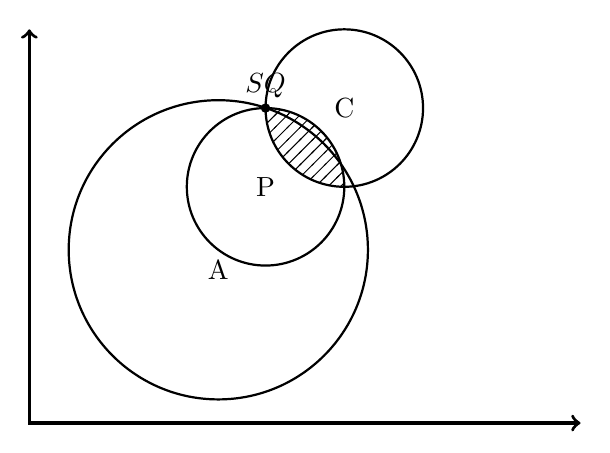
\begin{tikzpicture}
\begin{scope}[fill opacity=0.5]
\clip \thirdcircle;
\fill[pattern=flexible hatch, hatch distance=5.5pt, hatch thickness=0.35pt] \secondcircle;
\end{scope}
\fill[black] \ponto node[above]{$SQ$};
\draw[thick] \firstcircle node[below]{A};
\draw[thick] \secondcircle node{P};
\draw[thick] \thirdcircle node{C};
\draw[very thick,<->] (0,6) -- (0,1) -- (7,1);
\end{tikzpicture}
\end{document}
